%%%%%%%%%%%%%%%%%%%%%%%%%%%%%%%%%%%%%%%%%
% Minimalist Book Title Page 
% LaTeX Template
% Version 1.0 (27/12/12)
%
% This template has been downloaded from:
% http://www.LaTeXTemplates.com
%
% Original author:
% Peter Wilson (herries.press@earthlink.net)
%
% License:
% CC BY-NC-SA 3.0 (http://creativecommons.org/licenses/by-nc-sa/3.0/)
% 
% Instructions for using this template:
% This title page compiles as is. If you wish to include this title page in 
% another document, you will need to copy everything before 
% \begin{document} into the preamble of your document. The title page is
% then included using \titleTH within your document.
%
%%%%%%%%%%%%%%%%%%%%%%%%%%%%%%%%%%%%%%%%%

%----------------------------------------------------------------------------------------
%	PACKAGES AND OTHER DOCUMENT CONFIGURATIONS
%----------------------------------------------------------------------------------------

%\title{Microprocessor Architecture : Labo 1}

\documentclass{article}

\usepackage[utf8]{inputenc}
\usepackage[T1]{fontenc}
\usepackage[svgnames]{xcolor} % Required to specify font color
\usepackage{mathpazo}
\usepackage{floatrow}
\usepackage{geometry}%réglages mise en page
\geometry{%
a4paper, % note : l'option a4paper tuait la marge supérieure.
body={170mm,250mm}, %
left=25mm,top=25mm,right=25mm, %
headheight=21mm,headsep=7mm,
marginparsep=4mm,
marginparwidth=20mm, %
footnotesep=50mm
}
\usepackage{longtable}
\usepackage{pdflscape}
% allows for temporary adjustment of side margins
\usepackage{chngpage}
\usepackage{graphicx}
\usepackage{float}
\usepackage{color}
\usepackage{amssymb}

\newlength\longest

\newcommand*{\course}{\fbox{PROJ-H-402}} % Generic publisher logo

%----------------------------------------------------------------------------------------
%	TITLE PAGE
%----------------------------------------------------------------------------------------

\newcommand*{\titleTH}{\begingroup % Create the command for including the title page in the document
\raggedleft % Right-align all text
\vspace*{\baselineskip} % Whitespace at the top of the page

{\Large \textsc{Anthony Debruyn}}\\[0.167\textheight] % Author name

{\LARGE\bfseries Year Project}\\[\baselineskip] % First part of the title, if it is unimportant consider making the font size smaller to accentuate the main title

{\textcolor{Purple}{\Huge Wysiwyd}}\\[\baselineskip] % Main title which draws the focus of the reader

{\Large \textit{Wine cellar management,~~~~~~~~~~ \\almost without management}}\par % Tagline or further description

\vfill % Whitespace between the title block and the publisher

%\vspace*{30\baselineskip} % Whitespace at the bottom of the page
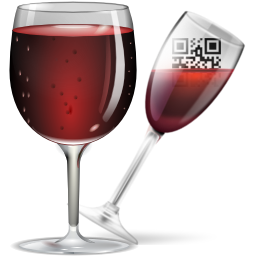
\includegraphics{Images/icon.png}

\vfill

{\large Gaëtan Podevijn \course}\par % Publisher and logo

%\vspace*{5\baselineskip} % Whitespace at the bottom of the page
\endgroup}

%----------------------------------------------------------------------------------------
%	BLANK DOCUMENT
%----------------------------------------------------------------------------------------

\begin{document} 

\thispagestyle{empty}

\titleTH % This command includes the title page

\newpage

%----------------------------------------------------------------------------------------
%	Introduction
%----------------------------------------------------------------------------------------

\section{Introduction}

Managing something composed of a large number of element can be tedious and complicated, event when you love doing it. This applies to oenologists as well when it comes to organising their wine cellar. This is where Wysiwyd enters in the game. The goal of Wysiwyd is to simplify the management of a wine cellar, to allow the oenologists and others to get the most of it.\\

Wysiwyd takes advantages of the new technologies available on the market, such as QR Code scanning and generating, NFC tags, to sort bottles. Photos of the bottles can be captured, so the user can see them right in the app as well. A search can be made on a lot of bottle properties to retrieve a desired bottle. The target OS is Android, leader on the smartphone market. The combination of the discovery of those technologies, the world of Android, the experience gained in mobile programming and design, is what makes this project fascinating.

%----------------------------------------------------------------------------------------
%	The App
%----------------------------------------------------------------------------------------

\section{The App}

\begin{quotation}
\center \emph{"What you scan is what you drink."\\ "Wysiwyd"}
\end{quotation}

\subsection{Functionalities}

\subsubsection{App Tour}

Once the app is loaded, the user has to choose between 2 actions. To \emph{scan a tag or a visual code}, or to \emph{list directly all the bottles}. Those 2 actions are symbolised by 2 bottles on the screen (see fig \ref{main_screen}).

\begin{figure}[H]
\begin{center}
	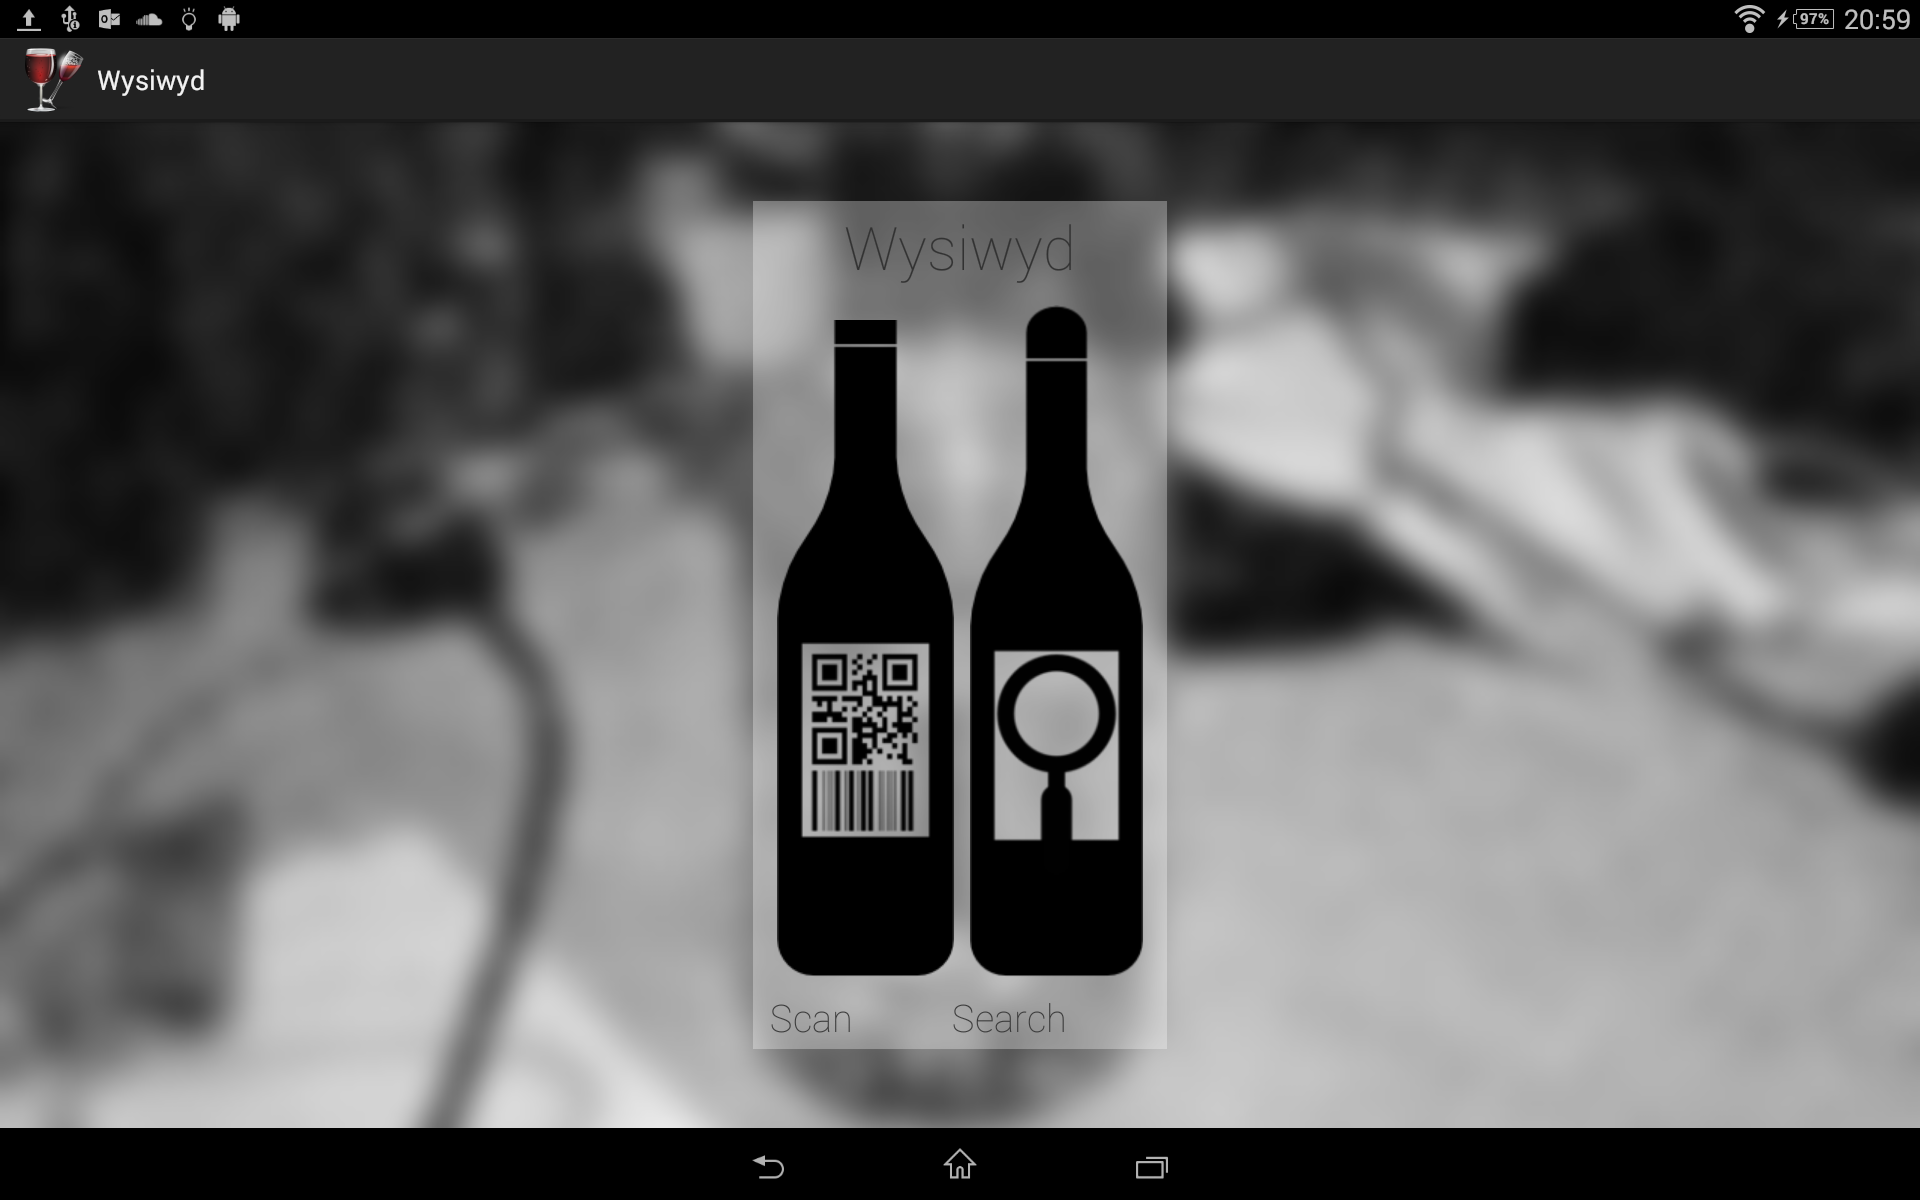
\includegraphics[width=\textwidth]{Images/MainActivity.png}
	\caption{The Main Screen.}
	\label{main_screen}
\end{center}
\end{figure}

If the user touches the first bottle, a new choice pops up: \emph{visual code}, or \emph{NFC tag} scan. This time, it is represented by glasses. The first one opens another app\footnote{Barcode Scanner, by ZXing Team} to scan a bottle bar code, or QR code\footnote{This visual code is the traduction of the number just below the bar code on wine bottles.}. If the user does not have this separate application, he can download it on the playstore for free. This app is not mandatory for this one to work. However, it is highly recommended, as it leads to easier management of the cellar.\\

Behind the glasses, and if the app has at least one image of a bottle, is a blurred picture of a bottle. This picture is one that the user took to illustrate his mobile database.


\begin{figure}[H]
\begin{center}
	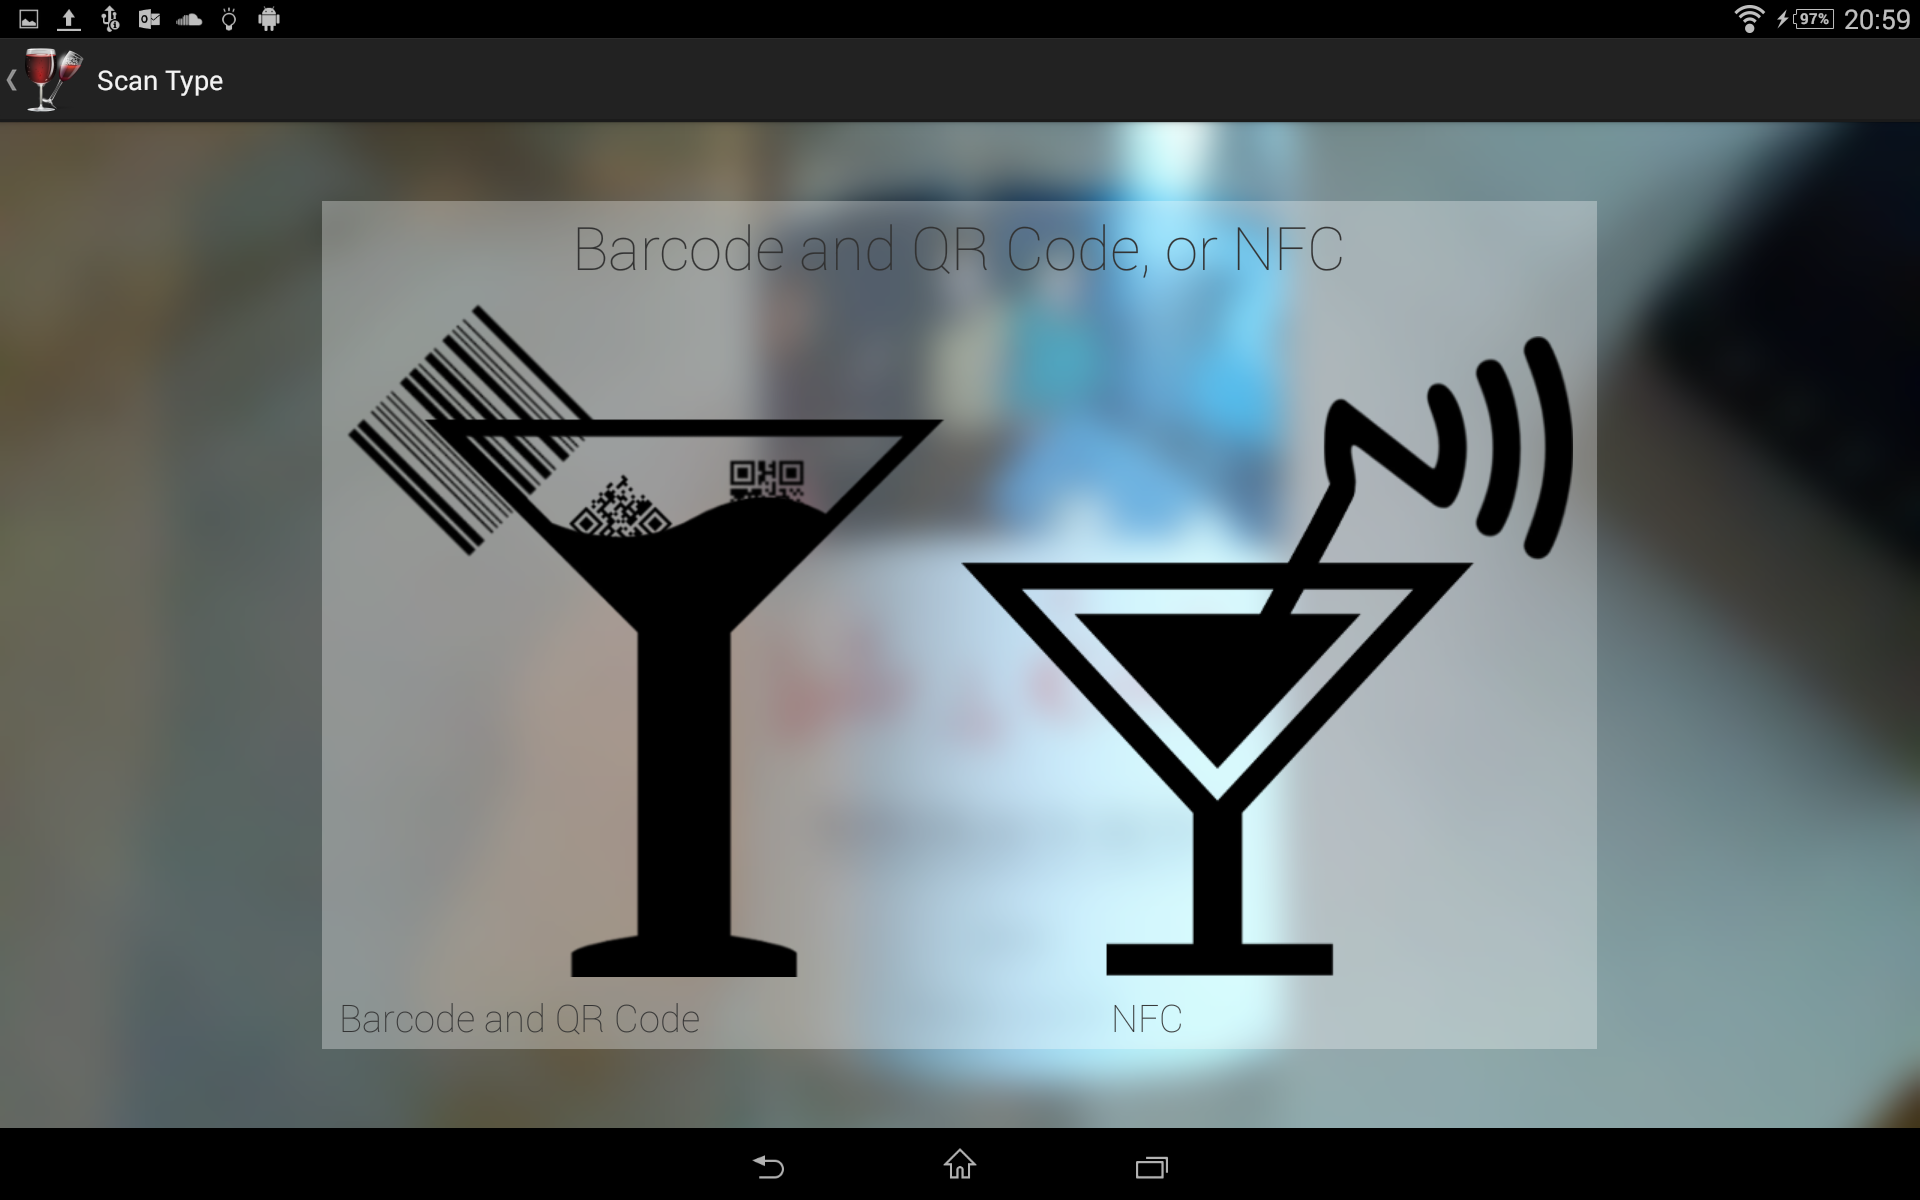
\includegraphics[width=\textwidth]{Images/ScanChoice.png}
	\caption{Visual Code, or NFC Tag ?}
	\label{scan_choice}
\end{center}
\end{figure}

By choosing the second glass, the user arrives in a third screen, only if NFC is available on the device (see fig. \ref{nfc_scan}). The NFC is in foreground mode as long as the user stays in this view. This means that no other app can intercept the NFC tag scan. Of course, if the user is not viewing this screen, the system still can intercept the tag if he places a bottle NFC tag near the NFC ship of the device. Then the system launches the app and directly lists the bottles with the corresponding code.

\begin{figure}[H]
\begin{center}
	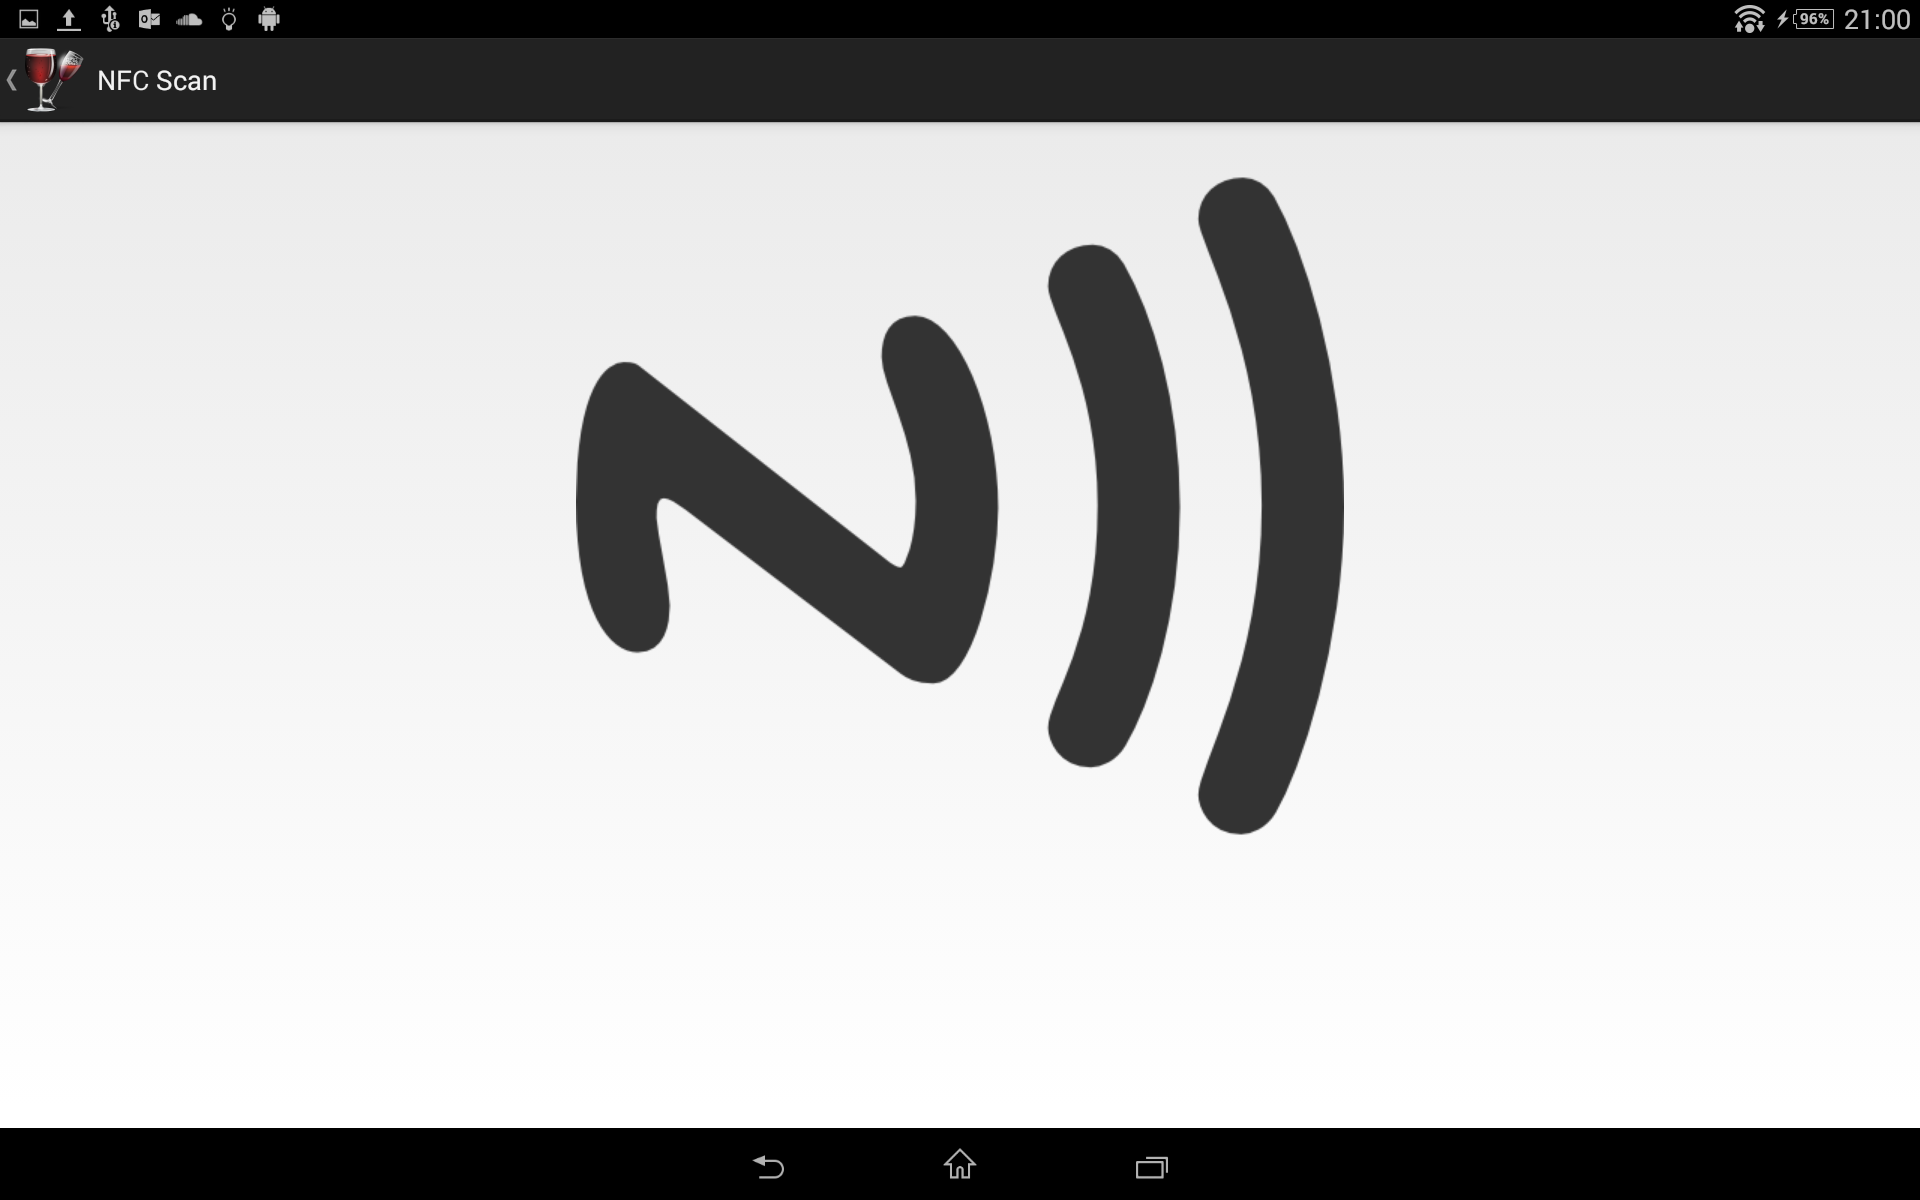
\includegraphics[width=\textwidth]{Images/NFCReaderActivity.png}
	\caption{NFC Tag Scan.}
	\label{nfc_scan}
\end{center}
\end{figure}

When the code has been captured, one way or another, the app shows a list of the corresponding bottles (fig. \ref{list_results}). If the user decides to add a bottle, the code will be copied in the corresponding text field automatically. If on figure \ref{main_screen} the user selected the second bottle, the screen on figure \ref{list_results} opens directly, displaying all the bottles in the order they were added to the database.

\begin{figure}[H]
\begin{center}
	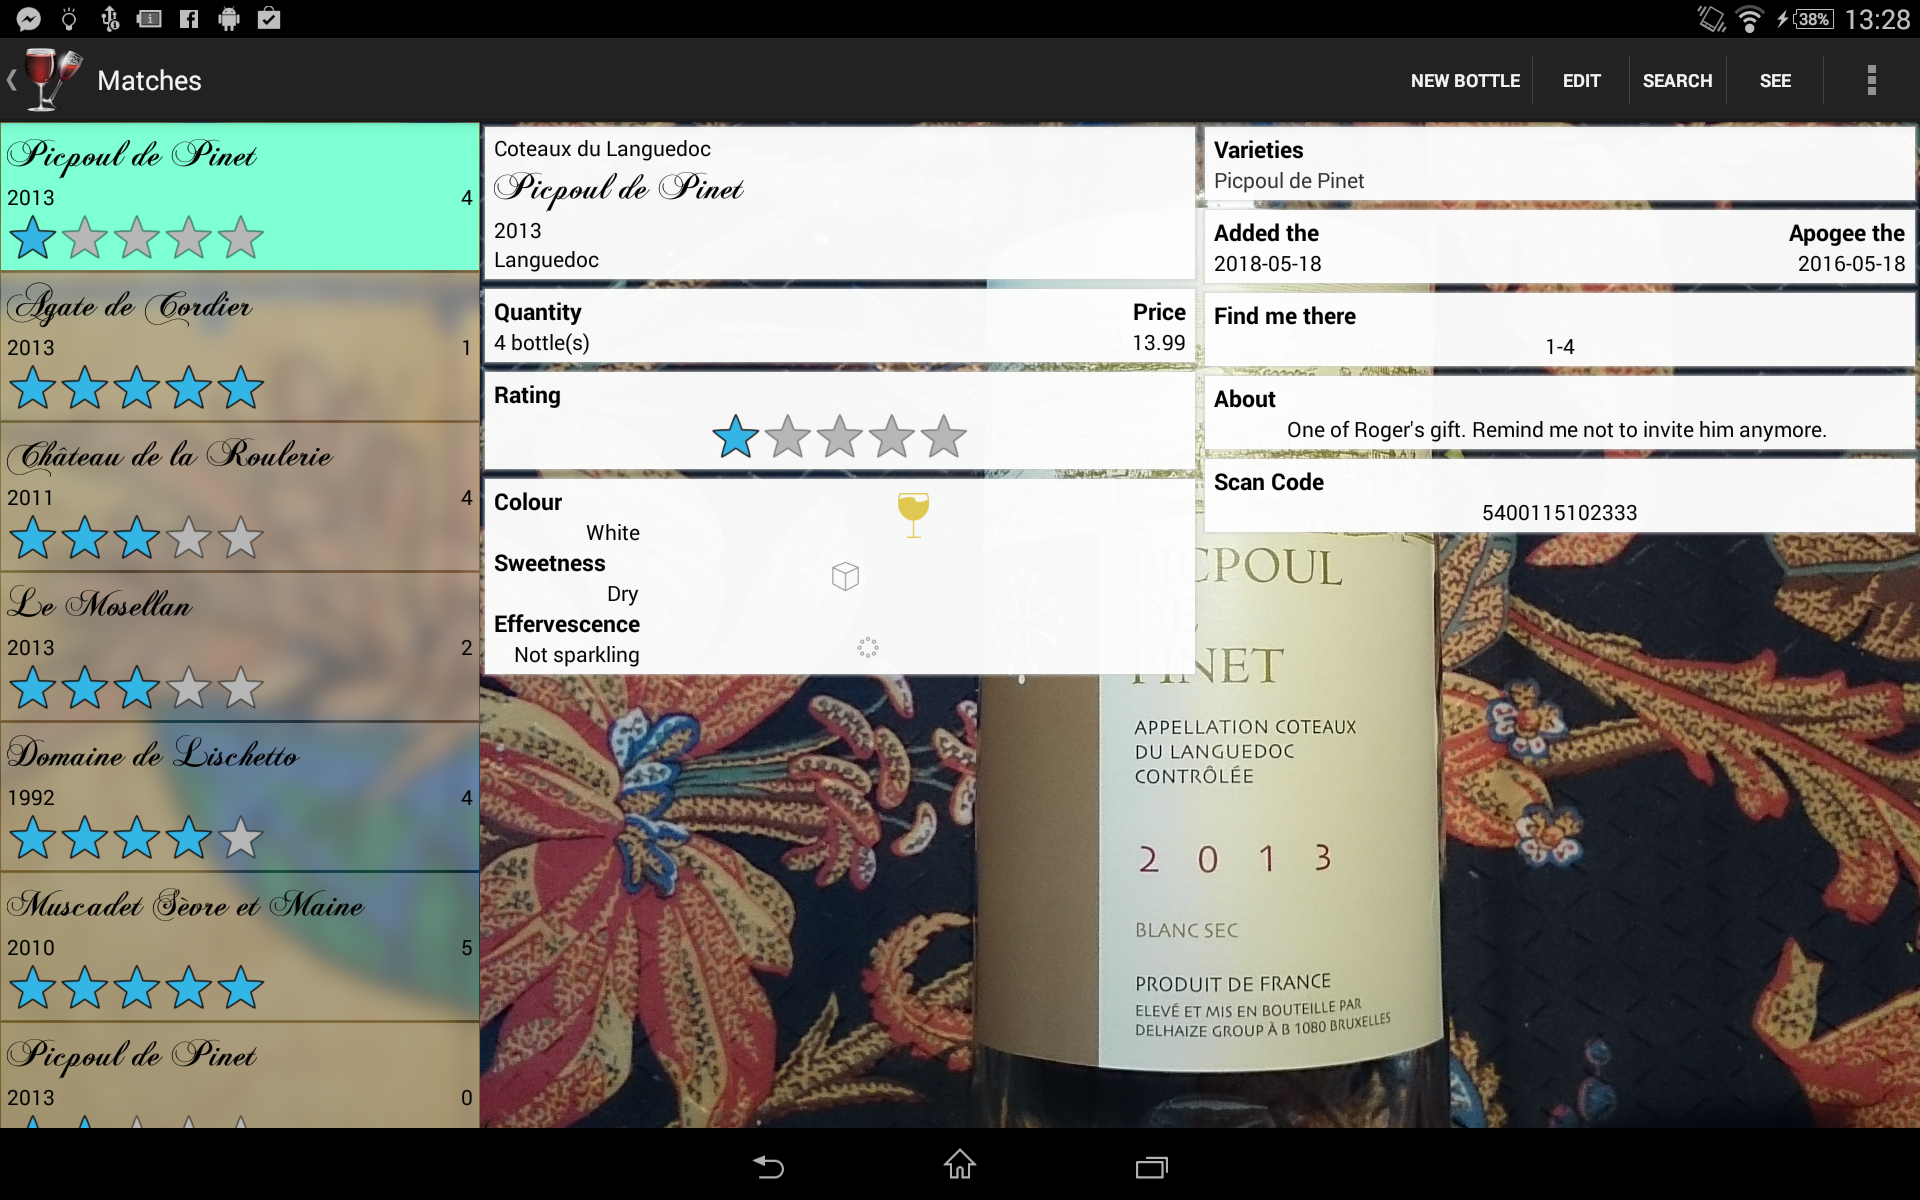
\includegraphics[width=\textwidth]{Images/ResultsActivity.png}
	\caption{List of results.}
	\label{list_results}
\end{center}
\end{figure}

On this figure, one can see all the details about a bottle. This is the view shown on a large screen device. On smaller devices, only one view is displayed at a time, either the details or the list.\\

Several buttons are aligned at the top right of the screen:
\begin{description}
\item[New Bottle:] To create a new bottle. Fill all the necessary text fields and other information, and click on \emph{Done}.
\item[Edit:] To edit an existing bottle. Click on \emph{Done} when finished.
\item[Search:] To search for bottles. Write down the desired properties, and click on \emph{Ok}. The list will refresh to display only the matching bottles.
\item[See:] To see the captured image of the bottle lying behind the view. This hides the details to show the background.
\end{description}

A long touch on the code section in the details will open the code exportation functionality. It will allow you to export the code to a QR code or/and to NFC tag. The layout of the corresponding view is similar to the figure \ref{scan_choice}. To generate a QR code and send it, the user is supposed to click on the "QR glass", while to write a NFC tag, the user has to push the "NFC glass". After generating the QR code, one can send it to a web service like Drive from Google, or email it.

\subsubsection{Adding a Bottle}



To add a bottle, several methods are available:

\begin{enumerate}
\item Add the new bottle directly by goin
\end{enumerate}

\section{The Database}

\subsection{The Entity Relationship Diagram}

\begin{figure}[H]
\begin{center}
	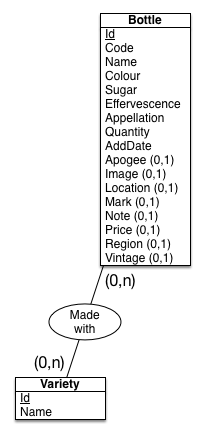
\includegraphics[scale=0.7]{../Entity Relationship DB diagram.png}
	\caption{The ERD.}
\end{center}
\end{figure}

\paragraph{Constraints}

\begin{itemize}
	\item If the effervescence is 0, then the vintage attribute is mandatory.
	\item Id, Code, Quantity, Vintage are a natural numbers.
	\item Price is a positive real number.
	\item Colour is a natural number in $\{ 0, 1, 2\}$.
	\item Sugar is a natural number in $\{0, 1, 2, 3\}$.
	\item Effervescence is a natural number in $\{0, 1, 2, 3\}$.
	\item Mark is a natural number in $\{1, 2, 3, 4, 5\}$.
	
\end{itemize}

\subsection{The Relational Model}

The translation of the ENR into the relational model:

\begin{description}
	\item[Bottle](\underline{Id}, Code, Name, Colour, Sugar, Effervescence, Appellation, Region, Vintage, Quantity, AddDate, \textit{Apogee}, \textit{Price}, \textit{Location}, \textit{Mark}, \textit{Image}, \textit{Note})
	
	\item[Variety](\underline{Id}, \underline{Name})
	
	\item[BottleVarieties](\underline{Bottle Id, Variety Id})\\ \\
	\emph{BottleVarieties.Bottle Id} foreign key to \emph{Bottle.Id}\\
	\emph{BottleVarieties.IdVariety} foreign key to \emph{Variety.Id}

\end{description}

\paragraph{Constraints}

\begin{itemize}
	\item If the type is "Champagne", then the Year attribute is not mandatory.
	\item The AddDate must be $\leq$ the current date.
	\item Id, Code, Quantity, Vintage are a natural numbers.
	\item Price is a positive real number.
	\item Colour is a natural number in $\{ 0, 1, 2\}$.
	\item Sugar is a natural number in $\{0, 1, 2, 3\}$.
	\item Effervescence is a natural number in $\{0, 1, 2, 3\}$.
	\item Mark is a natural number in $\{1, 2, 3, 4, 5\}$.
	\item For each Bottle Id in BottleVariety, there exists an Id in Bottle.
	\item For each Variety Id in BottleVariety, there exists an Id in Variety.
\end{itemize}

\paragraph{Remark}
Number are given to colours, varieties, etc. to allow the use of different string resources for different languages.

\subsection{Normalisation}

No normalisation was necessary.

\end{document}